\section{563 --- Binary Tree Tilt}
Given a binary tree, return the tilt of the \textbf{whole tree}.

The tilt of a \textbf{tree node} is defined as the \textbf{absolute difference} between the sum of all left subtree node values and the sum of all right subtree node values. Null node has tilt 0.

The tilt of the \textbf{whole tree} is defined as the sum of all nodes' tilt.

\paragraph{Example:}
\begin{flushleft}
\textbf{Input}: 
\begin{figure}[H]
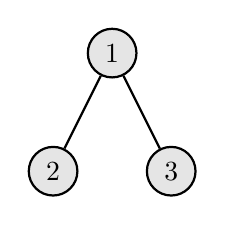
\begin{tikzpicture}
[every node/.style={draw, circle,minimum size=6mm, fill=gray!20!},
  node distance=8mm, thick]
\node{1}
child{node{2}}
child{node{3}};
\end{tikzpicture}
\end{figure}

\textbf{Output}: 1

\textbf{Explanation}: 

Tilt of node 2 : 0

Tilt of node 3 : 0

Tilt of node 1 : $\lvert 2-3\rvert = 1$

Tilt of binary tree : $0 + 0 + 1 = 1$
\end{flushleft}

\paragraph{Note:}

\begin{itemize}
\item The sum of node values in any subtree won't exceed the range of 32-bit integer.
\item All the tilt values won't exceed the range of 32-bit integer.
\end{itemize}

\subsection{Recursion}
\begin{itemize}
\item 递归函数应返回以某个node为根节点的tree的所有node的sum。
\item 分别对node的左右节点进行递归,将左右两个子树的sum的差的绝对值加入到最终结果中。
\end{itemize}

\setcounter{lstlisting}{0}
\begin{lstlisting}[style=customc, caption={Recursion}]
int findTilt( TreeNode* root )
{

    int ans = 0;

    dfs( root, ans );

    return ans;
}

//get the sum of all nodes in the tree
//rooted at node
//tilt is the by product of this function
int dfs( TreeNode* node, int& tilt )
{
    if( !node )
    {
        return 0;
    }

    //get left subtree sum
    int left = dfs( node->left, tilt );
    //get right subtree sum
    int right = dfs( node->right, tilt );

    tilt += abs( left - right );

    return node->val + left + right;
}
\end{lstlisting}